% Thesis proposal — follows Sample_Latex_Thesis2026.tex (Department of Mathematics, IU).
% Build: tectonic Thesis_Proposal.tex
\documentclass[12pt,a4paper,oneside]{book}
\usepackage{amssymb,amsthm,amsmath,amsfonts}
\renewcommand{\qedsymbol}{}
\usepackage{graphicx}
\usepackage[left= 3cm,right= 3cm,top=3cm,bottom=3cm]{geometry}
\usepackage{subcaption}
\usepackage{bm}
\usepackage{bbm}
\usepackage{makecell}
\usepackage{longtable}
\usepackage{setspace}
\usepackage{enumerate}
\usepackage{color}
\usepackage{multicol}
\usepackage{multirow}
\usepackage{indentfirst}
\usepackage{float}
\usepackage{framed}
\usepackage{hyperref}
\usepackage{fancyhdr}
\usepackage[utf8]{inputenc}
\usepackage{booktabs}
\usepackage{tabularx}
\usepackage{algorithm}
\usepackage{algorithmic}
\theoremstyle{definition}
\newtheorem{definition}{Definition}[section]
\newtheorem{theorem}{Theorem}[section]
\newtheorem{example}[definition]{Example}
\newtheorem{remark}[definition]{Remark}
\pagestyle{fancy}
\renewcommand{\headrulewidth}{0.1pt}
\fancyhf{}
\lhead{\nouppercase{\leftmark}}
\cfoot{\thepage}
\linespread{1.5}
\setlength{\emergencystretch}{2em}

\usepackage{tikz}
\usetikzlibrary{calc,positioning,arrows.meta}

\newcolumntype{L}{>{\raggedright\arraybackslash}X}
\newcommand{\TODO}[1]{\textcolor{red}{[#1]}}
\newcommand{\code}[1]{\texttt{#1}}
% Signature image overlaid on a signing line without moving the text.
% #1 offset from the left margin, #2 vertical shift of the image bottom, #3 height, #4 file.
\newcommand{\signature}[4]{\makebox[0pt][l]{\hspace{#1}\raisebox{#2}[0pt][0pt]{\includegraphics[height=#3]{#4}}}}

% Proposal metadata — fill in
\newcommand{\thesistitle}{LLM-GUIDED, DIMENSION-CONSTRAINED MONTE CARLO TREE SEARCH FOR FORMULAIC ALPHA DISCOVERY IN VN30F INDEX FUTURES}
\newcommand{\studentname}{NGUYEN TRUNG ANH}
\newcommand{\studentid}{MAMAIU22123}
\newcommand{\supervisor}{ASSOC. PROF. TRAN VU KHANH, Ph.D}

\begin{document}
	\begin{titlepage}
		\begin{center}
			\bf{VIETNAM NATIONAL UNIVERSITY – HO CHI MINH CITY}\\
			\bf{INTERNATIONAL UNIVERSITY}\\
			\bf{DEPARTMENT OF MATHEMATICS}\\
			\hfill
			\begin{center}
				
\includegraphics[scale=0.6]{logo.png}
			\end{center}
			\vspace*{1 cm}

			\bf  {THESIS PROPOSAL}
			\vspace*{1 cm}

			{\large\bf \thesistitle}\\
			\smallskip
			\bf {Submitted in partial fulfillment of the requirements for the degree of}\\
			\bf {BACHELOR OF SCIENCE}\\
			\bf {IN APPLIED MATHEMATICS}\\
			\bf {SPECIALIZATION IN FINANCIAL ENGINEERING }\\
			\bf {AND RISK MANAGEMENT}\\

			\vspace*{1 cm}
		\end{center}
		\begin{tabular}{ll}
			\bf Student's Name:  &\bf \studentname \\
			\bf Student's ID:   &\bf \studentid \\
			\bf Thesis Supervisor:&\bf \supervisor\\
		\end{tabular}

		\vspace*{1cm}
		\begin{center}
			{\bf Ho Chi Minh City, Vietnam}\\
			{\bf October 2026}\\
		\end{center}

		\newpage
		\thispagestyle{empty}
		\begin{center}
			\large\textbf{\thesistitle} \\
			\normalsize{By}\\
			\large{\studentname}\\
			\vskip10mm
			\normalsize{Submitted to DEPARTMENT OF MATHEMATICS,\\INTERNATIONAL UNIVERSITY, HO CHI MINH CITY\\ in partial fulfillment of requirements for the degree of\\
				BACHELOR OF SCIENCE \\
				IN APPLIED MATHEMATICS \\
				SPECIALIZATION IN FINANCIAL ENGINEERING  \\
				AND RISK MANAGEMENT}\\
			October 2026
			\vskip30mm
		\end{center}
        \signature{154pt}{-13pt}{61pt}{figures/signature_student.png}Signature of Student:
        \rule[0em]{26.7em}{0.5pt}
            \begin{flushright}\studentname \end{flushright}
		\vskip10mm
		\signature{158pt}{-16pt}{72pt}{figures/signature_supervisor.png}Certified by: \rule[0em]{30em}{0.5pt}
		\begin{flushright} \supervisor\\ Thesis Supervisor
		\end{flushright}
		\vskip10mm
		Approved by:
        \rule[0em]{30em}{0.5pt}
        \begin{flushright} ASSOC. PROF. MAI DUC THANH, Ph.D\\ ACTING HEAD OF DEPARTMENT OF MATHEMATICS
        \end{flushright}
	\end{titlepage}

	\newpage
	\thispagestyle{plain}
	\addcontentsline{toc}{chapter}{\numberline{}ABSTRACT}
	\begin{center}
		\large\textbf{\thesistitle} \\
		\normalsize{By}\\
		\large{\studentname}\\
		\vskip10mm
		\normalsize{Submitted to DEPARTMENT OF MATHEMATICS,\\INTERNATIONAL UNIVERSITY, HO CHI MINH CITY\\ in partial fulfillment of requirements for the degree of\\
			BACHELOR OF SCIENCE \\
			IN APPLIED MATHEMATICS \\
			SPECIALIZATION IN FINANCIAL ENGINEERING  \\
			AND RISK MANAGEMENT}\\
		\vspace*{0.5cm}
	\large\textbf{ABSTRACT}\\
	\end{center}
	\vskip2mm
Automated alpha-mining systems are usually judged by the strategies they produce, yet the best of many tried formulas looks good even when markets contain no exploitable structure. This thesis studies an LLM-guided Monte Carlo Tree Search system for VN30F1M index futures and asks what can actually be shown about such a system. Instead of testing individual alphas, the proposed protocol evaluates the discovery procedure itself: alpha sets produced in rolling search windows are traded on the following unseen months, compared with alternative procedures under an equal budget, and benchmarked against what the same procedure finds on placebo data and on data with a planted signal. A first version of the system illustrates the problem: only 1 of 171 candidates survived a robustness filter, and in-sample Sharpe ratios barely predicted performance on simulated paths.
\vskip10mm
\textbf{Keywords:} Formulaic alpha, Monte Carlo Tree Search, large language models, data snooping, walk-forward evaluation, permutation test, VN30F.

\newpage
\clearpage
\chapter*{ACKNOWLEDGEMENT}
\addcontentsline{toc}{chapter}{ACKNOWLEDGEMENT}

I would like to thank my supervisor, Assoc. Prof. Tran Vu Khanh, for guidance and feedback in shaping this proposal, and the Department of Mathematics, International University, for the education and support that made this work possible.

	\newpage
	\clearpage

	\mainmatter
	\tableofcontents
	\newpage
	\clearpage

\listoffigures
\newpage
\clearpage

\listoftables
\newpage
\clearpage

\chapter*{List of Abbreviations}
\addcontentsline{toc}{chapter}{List of Abbreviations}
\begin{description}
    \item[DSR] Deflated Sharpe Ratio
    \item[HMM] Hidden Markov Model
    \item[IC] Information Coefficient (Spearman correlation between a signal and the next-bar return)
    \item[LLM] Large Language Model
    \item[MCTS] Monte Carlo Tree Search
    \item[OOS] Out-of-Sample
    \item[SPA] Superior Predictive Ability (test)
    \item[TA] Technical Analysis
    \item[TSMOM] Time-Series Momentum
    \item[VN30F1M] VN30 index futures, front-month contract
\end{description}

\clearpage
\newpage
\clearpage

%══════════════════════════════════════════════════════════════════════════════
\chapter{INTRODUCTION}
\label{ch1}

\section{Motivation and Background}

Quantitative trading signals, or \emph{alphas}, are often written as explicit formulas over price and volume, such as the 101 alphas published by Kakushadze \cite{kakushadze2016}. Because the space of such formulas is combinatorial, a growing body of work searches it automatically, first with genetic programming \cite{koza1992} and reinforcement learning \cite{yu2023,xu2024}, and more recently with large language models (LLMs), alone \cite{wang2023,tang2025} or combined with Monte Carlo Tree Search (MCTS) \cite{ren2024,shi2026}.

This thesis builds on such a system for VN30F1M, the front-month VN30 index futures contract and the most liquid derivative in Vietnam. An LLM proposes the structure of a strategy, an MCTS completes the formula inside a grammar where every node carries a physical dimension, and each candidate is scored by a backtest that models the fees, margin and rollover of the Vietnamese derivatives market.

\section{Literature Review}
\label{sec:litreview}

\subsection{Automated and LLM-Based Alpha Mining}

Kakushadze \cite{kakushadze2016} published 101 formulaic alphas used in practice, built from ranks, delays, differences, correlations and rolling extrema. The space of such formulas has been searched with genetic programming \cite{koza1992}, with reinforcement learning that generates sets of alphas working well in combination \cite{yu2023}, and with tree search \cite{xu2024,ren2024}, building on the UCT rule of MCTS \cite{kocsis2006,browne2012}. More recently, LLMs turn research ideas into alpha expressions \cite{wang2023}, act as agents that avoid duplicating existing alphas \cite{tang2025}, or refine formulas inside MCTS using backtest feedback \cite{shi2026}, in the spirit of self-refinement \cite{madaan2023}.

\subsection{How Alpha-Mining Systems Are Evaluated}

The studies above share an evaluation protocol. The system is run on a training period, the alphas it produces are combined, and the combination is evaluated on a later test period: 2011--2020 versus 2021--2024 in \cite{shi2026}, 2010--2019 versus 2021--2022 in \cite{ren2024}, 2009--2018 versus 2021--2023 in \cite{xu2024}. Performance is measured by the information coefficient, complemented in \cite{shi2026,ren2024} by trading simulations, and compared against baseline mining methods; \cite{shi2026} also ablates each component of its framework. All of these studies are cross-sectional: each test day contributes hundreds of stocks, so even a small information coefficient can be estimated precisely. Industry practice follows the same logic; according to its public documentation, WorldQuant BRAIN evaluates submitted alphas on a two-year out-of-sample period hidden from the researcher.

\subsection{Data Snooping and Statistical Significance}

When a model is selected from a search, its performance must be compared with the distribution of the \emph{best} of all tried models: the Reality Check of White \cite{white2000} and the SPA test of Hansen \cite{hansen2005}. Aronson \cite{aronson2006} applied such tests and Monte Carlo permutations to technical trading rules, and Masters \cite{masters2020} extends permutation tests to entire trading-system development procedures. Backtested Sharpe ratios can be haircut for the number of trials \cite{harvey2015,harvey2016} or deflated \cite{bailey2014}, and the probability of backtest overfitting can be estimated \cite{bailey2017}. Lo \cite{lo2002} gives the sampling distribution of the Sharpe ratio, which fixes how much data is needed to detect an edge. Synthetic data with known properties let one check whether a method recovers what is there \cite{lopezdeprado2018,arian2024}; regime-switching paths can be produced with hidden Markov models and block bootstrapping \cite{hamilton1989,rabiner1989,kunsch1989}.

\subsection{Research Gap}

\begin{enumerate}
  \item Evaluation protocols for alpha-mining systems were developed for cross-sectional equities. For a single instrument the same protocol has far less statistical power, and the literature reviewed here does not address how to compensate.
  \item Published systems are compared with each other but not with what the same procedure finds when no signal exists, nor checked for their ability to recover a known signal.
  \item No study evaluates an LLM-guided search for directional signals on Vietnamese index futures.
\end{enumerate}

\section{Problem Statement}

A discovery system of this kind evaluates thousands of formulas and keeps the best. The best of many trials looks good even when the data contain no exploitable structure, so a strong backtest of a selected alpha does not show that the system has discovered anything \cite{white2000,harvey2016,harvey2015}. The problem is sharper for a single instrument than for the cross-sectional stock universes studied in most alpha-mining papers: with one contract, evidence accumulates only over time, and one or two years of out-of-sample returns cannot separate a modest edge from luck \cite{lo2002}.

The evaluation currently used by the system---filtering each selected alpha through robustness tests on simulated paths---shares this weakness. It produced the result that motivates this thesis: of 171 candidates, one survived, and the in-sample performance of a candidate said little about how it behaved on simulated paths (Chapter~\ref{ch4}). Neither outcome tells us whether the system works. What is missing is a question that can be answered, and a test that answers it.

\section{Research Questions}

The object of study is the discovery \emph{procedure}, not any individual alpha. Each question is answered by comparing the out-of-sample performance of the alpha \emph{sets} produced by different procedures given the same data and the same evaluation budget.

\begin{enumerate}
  \item[\textbf{RQ1.}] \textbf{Role of the LLM.} Does LLM + MCTS produce alpha sets with higher out-of-sample performance than MCTS without LLM blueprints, the LLM without search, and random search?
  \item[\textbf{RQ2.}] \textbf{Search space.} Do primitive time-series operators produce better out-of-sample alpha sets than hand-crafted technical indicators?
  \item[\textbf{RQ3.}] \textbf{Evidence of discovery.} Is the out-of-sample performance of the full system higher than what the same procedure achieves on placebo data without predictable structure, and does the procedure recover a signal deliberately planted in synthetic data?
\end{enumerate}

The thesis therefore aims to build an evaluation protocol that answers these questions, and to report every outcome, including negative ones.

\section{Scope}

The study covers one instrument, VN30F1M, using one-minute to one-hour OHLCV bars from the broker DNSE between 13/08/2018 and 31/12/2025. Signals are directional (long, short or flat). Cross-sectional stock portfolios and live trading are out of scope. The discovery system is taken largely as given; the contribution lies in how it is evaluated.

The rest of the proposal is organized as follows. Chapter \ref{ch3} briefly describes the existing system and its current evaluation, then presents the proposed protocol. Chapter \ref{ch4} reports preliminary results, and Chapter \ref{ch5} summarises the expected contributions and the work plan.

%══════════════════════════════════════════════════════════════════════════════
\chapter{METHODOLOGY}
\label{ch3}

\section{The Existing Discovery System}

The system (Figure~\ref{fig:arch}) has three parts. An LLM proposes a \emph{blueprint}, an expression with open slots such as \code{ts\_zscore(sub(?, ts\_mean(?)))}; a semantic compiler parses it and returns errors to the LLM for self-correction \cite{madaan2023}. An MCTS fills the slots with operators and inputs from a grammar in which every node carries a dimension---price, volume, ratio or boolean---so that dimensionally meaningless formulas, such as price plus volume, are never generated. Each formula is turned into long, short or flat positions and scored by a backtest that models VN30F1M trading: execution one bar after the signal, netting fees, initial and maintenance margin with margin calls, and rollover at expiry. The combination of LLM structure proposals with a dimension-typed grammar, applied to directional signals on a single futures contract, is what distinguishes the system from the studies in Section~\ref{sec:litreview}.

\begin{figure}[H]
\centering
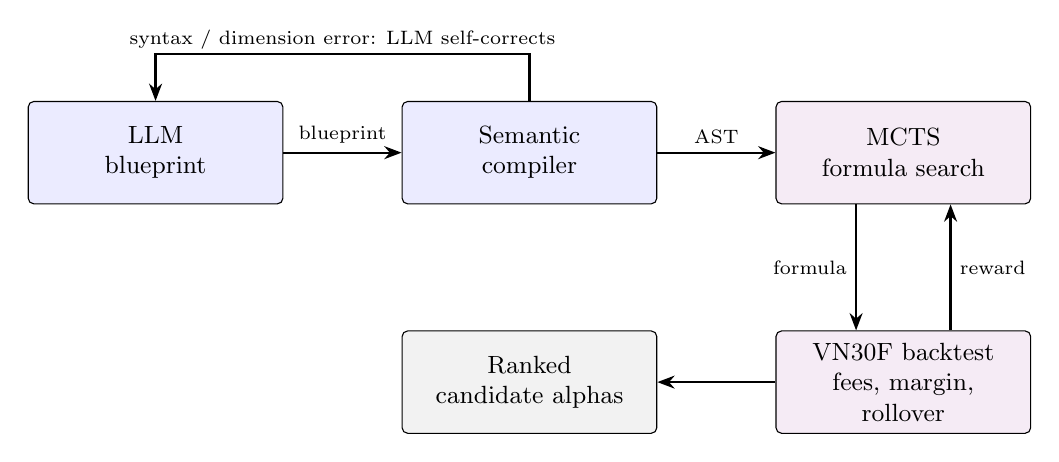
\begin{tikzpicture}[
  node distance=1.6cm and 1.5cm,
  box/.style={draw, rounded corners=2pt, align=center, font=\small\setstretch{1.0}, minimum height=1.3cm, text width=3.0cm, fill=#1},
  box/.default={white},
  arr/.style={-{Stealth[length=2.2mm]}, thick},
  lbl/.style={font=\scriptsize, align=center, fill=white, inner sep=1pt}]
  \node[box=blue!8] (llm) {LLM\\blueprint};
  \node[box=blue!8, right=of llm] (comp) {Semantic\\compiler};
  \node[box=violet!8, right=of comp] (mcts) {MCTS\\formula search};
  \node[box=violet!8, below=of mcts] (bt) {VN30F backtest\\fees, margin,\\rollover};
  \node[box=gray!10, left=of bt] (out) {Ranked\\candidate alphas};
  \draw[arr] (llm) -- node[above, lbl, yshift=2pt]{blueprint} (comp);
  \draw[arr] (comp) -- node[above, lbl, yshift=2pt]{AST} (mcts);
  \draw[arr] (comp.north) -- ++(0,0.6) -| node[pos=0.25, above, lbl]{syntax / dimension error: LLM self-corrects} (llm.north);
  \draw[arr] ([xshift=-6mm]mcts.south) -- node[left, lbl, xshift=-2pt]{formula} ([xshift=-6mm]bt.north);
  \draw[arr] ([xshift=6mm]bt.north) -- node[right, lbl, xshift=2pt]{reward} ([xshift=6mm]mcts.south);
  \draw[arr] (bt) -- (out);
\end{tikzpicture}
\caption{The existing discovery system}
\label{fig:arch}
\end{figure}

\section{Current Evaluation and Its Limitations}
\label{sec:current}

At present, the best candidate found by MCTS on 2020--2024 is filtered through three tests on 500 synthetic price paths generated by a three-state hidden Markov model with block bootstrapping: a ruin-rate limit, a positive Kelly fraction with sufficient profit per trade relative to costs, and a minimum return relative to a savings rate and to buy-and-hold. This evaluation cannot answer whether the system works, for four reasons:
\begin{enumerate}
  \item \textbf{No null distribution.} The object evaluated is the best of many trials. Without knowing how good the best trial looks when there is nothing to find, a good result cannot be distinguished from luck \cite{white2000,harvey2015}.
  \item \textbf{No independent data.} The synthetic paths are resampled from the same history that was searched, so passing the filter is not independent evidence. The thresholds are economic criteria with no stated error rate.
  \item \textbf{Insufficient out-of-sample evidence.} There is no out-of-sample period at all. Even a single held-out year would not suffice: for daily returns, the standard error of an annualised Sharpe ratio is close to $1/\sqrt{T}$ for $T$ years \cite{lo2002}, so one year can only confirm Sharpe ratios above about 2.
  \item \textbf{No comparison.} Without alternative procedures run under the same conditions, no result can be attributed to the LLM, to MCTS or to the operator set.
\end{enumerate}

\section{Proposed Evaluation Protocol}
\label{sec:protocol}

\subsection{Unit of Evaluation}

Following \cite{shi2026,ren2024,xu2024}, the procedure is run on a search window and the alphas it produces are combined into one strategy, which is then traded on a later, unseen evaluation window. The combination is fixed in advance: the target positions of the $k = 5$ highest-ranked alphas are averaged with equal weights. The primary metric is the annualised Sharpe ratio of the daily net returns of this strategy, collected over all evaluation windows; the information coefficient, Calmar ratio and turnover are reported as secondary metrics. Individual alphas are never tested in isolation.

\subsection{Walk-Forward Evaluation}

To gain statistical power from time, the procedure is re-run on rolling windows: two years of search followed by six months of evaluation, rolled forward by six months (Figure~\ref{fig:wf}). Eleven windows yield five and a half years of out-of-sample returns, from July 2020 to December 2025, enough to confirm Sharpe ratios of about $2/\sqrt{5.5} \approx 0.85$ at conventional significance \cite{lo2002}. Because MCTS and the rollouts are randomised, each configuration is run with five random seeds, and the mean and dispersion across seeds are reported.

\begin{figure}[H]
\centering
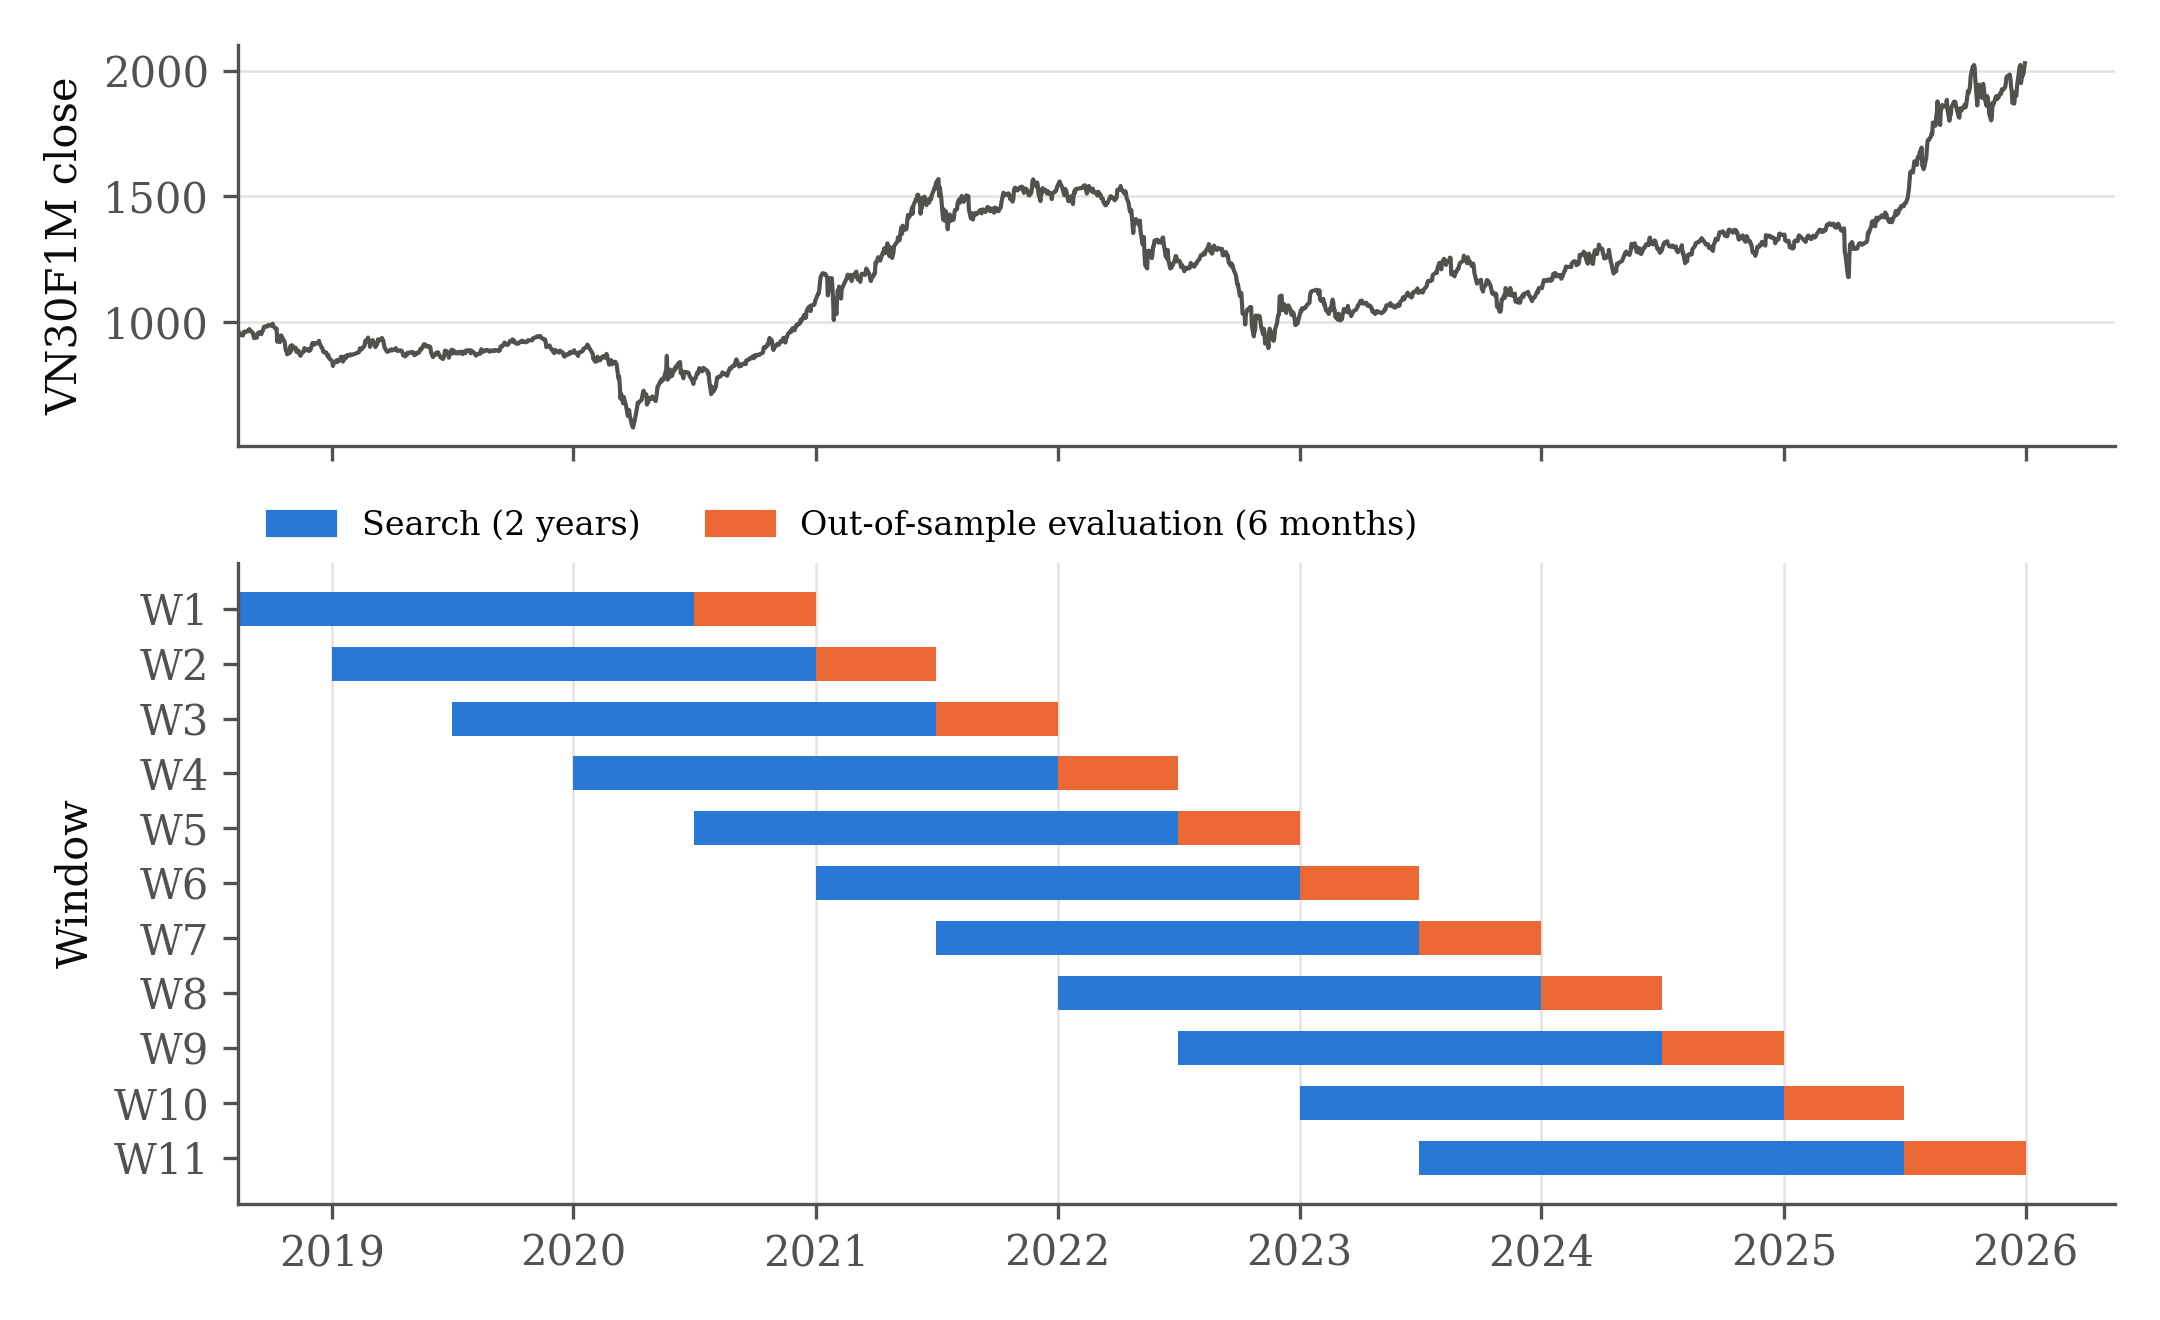
\includegraphics[width=0.82\textwidth]{figures/walk_forward.png}
\caption{Walk-forward windows: two-year search, six-month out-of-sample evaluation}
\label{fig:wf}
\end{figure}

\subsection{Configurations Compared (RQ1, RQ2)}

All configurations in Table~\ref{tab:configs} receive the same number of backtest evaluations in each window. LLM blueprints are generated once and frozen, so that every configuration and window uses the same set.

\begin{table}[H]
\centering
\caption{Configurations compared under an equal evaluation budget}
\label{tab:configs}
\begin{tabularx}{\textwidth}{lLl}
\toprule
\textbf{Configuration} & \textbf{Description} & \textbf{RQ} \\
\midrule
LLM + MCTS & Full system & 1, 2, 3 \\
MCTS only & MCTS from an empty tree, no blueprints & 1 \\
LLM only & LLM writes complete formulas, no search & 1 \\
Random search & Random dimension-valid formulas & 1 \\
TA indicators & LLM + MCTS over technical indicators instead of primitive operators & 2 \\
Buy-and-hold & Always long & reference \\
TSMOM & Time-series momentum \cite{moskowitz2012}, adapted to intraday bars & reference \\
\bottomrule
\end{tabularx}
\end{table}

\subsection{Placebo Test (RQ3, Negative Control)}

To learn what the procedure finds when there is nothing to find, the full walk-forward run is repeated on $K$ placebo datasets in which the predictability of returns has been destroyed. The primary placebo permutes bar returns within each search window \cite{aronson2006,masters2020}; a variant randomly flips the sign of whole trading days, which also preserves volatility clustering. Because each placebo run repeats the entire procedure, the test evaluates the discovery procedure as a whole, in the sense of Masters \cite{masters2020}. The p-value is the fraction of runs, real data included, whose out-of-sample Sharpe ratio is at least that of the real run. With $K = 19$, the smallest attainable p-value is $1/20 = 0.05$; a reduced search budget is used for placebo runs if computation requires it.

\subsection{Planted-Signal Test (RQ3, Positive Control)}

To check that a negative result would reflect the market rather than a blind procedure, a known formula that the grammar can express is planted in placebo returns with a controlled strength, measured by its information coefficient (for example 0.01, 0.02 and 0.05). For each strength, the protocol records whether the procedure recovers the planted formula, or one highly correlated with it, and the out-of-sample Sharpe ratio it achieves. This follows the use of synthetic controlled environments to assess backtesting methods \cite{lopezdeprado2018,arian2024}.

\subsection{Statistical Tests}

Differences between configurations are tested with the SPA test \cite{hansen2005}, using random search as the benchmark, on the out-of-sample daily returns. The final strategy of the full system is additionally assessed with the Deflated Sharpe Ratio \cite{bailey2014}, taking as the number of trials the total number of formulas evaluated across windows and directions. The existing HMM-based tests are kept only to describe the risk of strategies that already passed the tests above; because their paths are resampled from the searched history, they are not evidence of an edge.

%══════════════════════════════════════════════════════════════════════════════
\chapter{PRELIMINARY RESULTS}
\label{ch4}

A first version of the system, searching over technical indicators, produced 171 candidate strategies: 22 written directly by the LLM and 149 found by MCTS. Each was evaluated with the current filter of Section~\ref{sec:current}. Table~\ref{tab:prelim} summarises the outcome.

\begin{table}[H]
\centering
\caption{Filter outcome of the first-generation strategies}
\label{tab:prelim}
\setstretch{1.1}
\begin{tabular}{lrrr}
\toprule
 & \textbf{LLM only} & \textbf{MCTS} & \textbf{Total} \\
\midrule
Rejected at tier 1 (ruin) & 22 & 140 & 162 (94.7\%) \\
Rejected at tier 2 (costs) & 0 & 4 & 4 \\
Rejected at tier 3 (opportunity cost) & 0 & 4 & 4 \\
\textbf{Passed all tiers} & \textbf{0} & \textbf{1} & \textbf{1} \\
\midrule
Median in-sample Sharpe ratio & 1.48 & 0.99 & \\
\bottomrule
\end{tabular}
\end{table}

These results illustrate the limitations of Section~\ref{sec:current} rather than answer the research questions:
\begin{enumerate}
  \item The correlation between in-sample Sharpe ratios and mean Sharpe ratios on simulated paths was only 0.19--0.24. For MCTS strategies, the historical Sharpe ratio sat at a median percentile of 96--100\% among the simulated paths: performance was specific to the one path that had been searched.
  \item Strategies written directly by the LLM had the highest in-sample Sharpe ratios, yet none survived.
  \item The single surviving alpha lay close to the acceptance boundary: an earlier version of the filter rejected it with 100 simulated paths and accepted it with 300.
\end{enumerate}
None of these observations can say whether the system finds more than chance; that requires the protocol of Section~\ref{sec:protocol}.

%══════════════════════════════════════════════════════════════════════════════
\chapter{CONCLUSION AND FUTURE STUDY}
\label{ch5}

\section{Expected Contributions}

\begin{enumerate}
  \item An evaluation protocol for automated alpha discovery on a single instrument, combining walk-forward evaluation of alpha sets, equal-budget comparison of procedures, placebo calibration and planted-signal checks.
  \item Evidence on the value of LLM guidance (RQ1) and of primitive operators over technical indicators (RQ2) for VN30F1M.
  \item An answer to whether the system finds more than chance on VN30F1M (RQ3). A negative answer, supported by a successful planted-signal test, is itself a result: it would indicate that, after costs, the market offers no edge expressible in the grammar that the procedure can detect.
\end{enumerate}

\section{Research Plan}

\begin{table}[H]
\centering
\caption{Work plan}
\label{tab:plan}
\begin{tabularx}{\textwidth}{lL}
\toprule
\textbf{Period} & \textbf{Tasks} \\
\midrule
Month 1 & Complete the primitive-operator pipeline; make the data window an input; fix random seeds; run the planted-signal test on one bar frequency. \\
Month 2 & Implement the walk-forward loop, alpha combination and placebo datasets; implement the baseline configurations. \\
Month 3 & Run all configurations on the real data (RQ1, RQ2). \\
Month 4 & Run the placebo and planted-signal tests (RQ3); SPA and DSR; robustness analysis. \\
Month 5 & Analyse results and write the thesis. \\
Month 6 & Revise and prepare the defence. \\
\bottomrule
\end{tabularx}
\end{table}

\section{Risks and Mitigation}

If the system does not beat placebo, the thesis reports a well-founded negative result, provided the planted-signal test succeeds; that test is run first so that a defective procedure can be fixed early. Placebo runs are costly, so a reduced search budget may be used for them. Finally, an LLM trained on recent data may know how the market moved \cite{shi2026}; the LLM only proposes structure, its blueprints are frozen, and the MCTS-only configuration provides a comparison free of this concern.

%══════════════════════════════════════════════════════════════════════════════
\addcontentsline{toc}{chapter}{Bibliography}
\begin{thebibliography}{99}

\bibitem{arian2024}
Arian, H. R., Norouzi Mobarekeh, D., \& Seco, L. A. (2024). Backtest overfitting in the machine learning era: A comparison of out-of-sample testing methods in a synthetic controlled environment. \textit{Knowledge-Based Systems}, 305.

\bibitem{aronson2006}
Aronson, D. (2006). \textit{Evidence-based technical analysis: Applying the scientific method and statistical inference to trading signals}. Wiley.

\bibitem{bailey2014}
Bailey, D. H., \& L\'opez de Prado, M. (2014). The deflated Sharpe ratio: Correcting for selection bias, backtest overfitting and non-normality. \textit{The Journal of Portfolio Management}, 40(5), 94-107.

\bibitem{bailey2017}
Bailey, D. H., Borwein, J. M., L\'opez de Prado, M., \& Zhu, Q. J. (2017). The probability of backtest overfitting. \textit{Journal of Computational Finance}, 20(4), 39-69.

\bibitem{browne2012}
Browne, C. B., Powley, E., Whitehouse, D., Lucas, S. M., Cowling, P. I., Rohlfshagen, P., Tavener, S., Perez, D., Samothrakis, S., \& Colton, S. (2012). A survey of Monte Carlo tree search methods. \textit{IEEE Transactions on Computational Intelligence and AI in Games}, 4(1), 1-43.

\bibitem{hamilton1989}
Hamilton, J. D. (1989). A new approach to the economic analysis of nonstationary time series and the business cycle. \textit{Econometrica}, 57(2), 357-384.

\bibitem{hansen2005}
Hansen, P. R. (2005). A test for superior predictive ability. \textit{Journal of Business \& Economic Statistics}, 23, 365-380.

\bibitem{harvey2015}
Harvey, C. R., \& Liu, Y. (2015). Backtesting. \textit{The Journal of Portfolio Management}, 42(1), 13-28.

\bibitem{harvey2016}
Harvey, C. R., Liu, Y., \& Zhu, H. (2016). \ldots and the cross-section of expected returns. \textit{The Review of Financial Studies}, 29(1), 5-68.

\bibitem{kakushadze2016}
Kakushadze, Z. (2016). 101 formulaic alphas. \textit{Wilmott}, 2016(84), 72-80.

\bibitem{kocsis2006}
Kocsis, L., \& Szepesv\'ari, C. (2006). Bandit based Monte-Carlo planning. In \textit{Machine Learning: ECML 2006}, Lecture Notes in Computer Science, vol. 4212 (pp. 282-293). Springer.

\bibitem{koza1992}
Koza, J. R. (1992). \textit{Genetic programming: On the programming of computers by means of natural selection}. MIT Press.

\bibitem{kunsch1989}
K\"unsch, H. R. (1989). The jackknife and the bootstrap for general stationary observations. \textit{The Annals of Statistics}, 17(3), 1217-1241.

\bibitem{lo2002}
Lo, A. W. (2002). The statistics of Sharpe ratios. \textit{Financial Analysts Journal}, 58(4), 36-52.

\bibitem{lopezdeprado2018}
L\'opez de Prado, M. (2018). \textit{Advances in financial machine learning}. Wiley.

\bibitem{madaan2023}
Madaan, A., Tandon, N., Gupta, P., Hallinan, S., Gao, L., Wiegreffe, S., Alon, U., Dziri, N., Prabhumoye, S., Yang, Y., Gupta, S., Majumder, B. P., Hermann, K., Welleck, S., Yazdanbakhsh, A., \& Clark, P. (2023). Self-Refine: Iterative refinement with self-feedback. In \textit{Advances in Neural Information Processing Systems 36 (NeurIPS 2023)}.

\bibitem{masters2020}
Masters, T. (2020). \textit{Permutation and randomization tests for trading system development: Algorithms in C++}. Independently published.

\bibitem{moskowitz2012}
Moskowitz, T. J., Ooi, Y. H., \& Pedersen, L. H. (2012). Time series momentum. \textit{Journal of Financial Economics}, 104(2), 228-250.

\bibitem{rabiner1989}
Rabiner, L. R. (1989). A tutorial on hidden Markov models and selected applications in speech recognition. \textit{Proceedings of the IEEE}, 77(2), 257-286.

\bibitem{ren2024}
Ren, T., Zhou, R., Jiang, J., Liang, J., Wang, Q., \& Peng, Y. (2024). RiskMiner: Discovering formulaic alphas via risk seeking Monte Carlo tree search. In \textit{Proceedings of the 5th ACM International Conference on AI in Finance (ICAIF '24)}.

\bibitem{shi2026}
Shi, Y., Duan, Y., \& Li, J. (2026). Navigating the alpha jungle: An LLM-powered MCTS framework for formulaic factor mining. In \textit{Proceedings of the AAAI Conference on Artificial Intelligence}. arXiv:2505.11122.

\bibitem{tang2025}
Tang, Z., Chen, Z., Yang, J., Mai, J., Zheng, Y., Wang, K., Chen, J., \& Lin, L. (2025). AlphaAgent: LLM-driven alpha mining with regularized exploration to counteract alpha decay. \textit{arXiv preprint arXiv:2502.16789}.

\bibitem{wang2023}
Wang, S., Yuan, H., Zhou, L., Ni, L. M., Shum, H.-Y., \& Guo, J. (2023). Alpha-GPT: Human-AI interactive alpha mining for quantitative investment. \textit{arXiv preprint arXiv:2308.00016}.

\bibitem{white2000}
White, H. (2000). A reality check for data snooping. \textit{Econometrica}, 68(5), 1097-1126.

\bibitem{xu2024}
Xu, F., Yin, Y., Zhang, X., Liu, T., Jiang, S., \& Zhang, Z. (2024). Alpha$^2$: Discovering logical formulaic alphas using deep reinforcement learning. \textit{arXiv preprint arXiv:2406.16505}.

\bibitem{yu2023}
Yu, S., Xue, H., Ao, X., Pan, F., He, J., Tu, D., \& He, Q. (2023). Generating synergistic formulaic alpha collections via reinforcement learning. In \textit{Proceedings of the 29th ACM SIGKDD Conference on Knowledge Discovery and Data Mining}.

\end{thebibliography}

\newpage

\appendix
\section*{Appendix A: Access to Source Code}

The source code is available at \url{https://github.com/NguyenTrungAnh-ultra/alpha_farm}.

\end{document}
